\documentclass[a4paper,twoside]{article}
\usepackage[utf8]{inputenc}
\usepackage[T1]{fontenc}
\usepackage{enumerate}
\usepackage{graphicx}

\newcommand{\Ra}{$\Rightarrow$}
%Defining \vec to make a symbol bold
\if@mathematic
   \def\vec#1{\ensuremath{\mathbf{#1}}}
\else
   \def\vec#1{\ensuremath{\mathchoice{\mbox{\boldmath$\displaystyle#1$}}
                              {\mbox{\boldmath$\textstyle#1$}}
                              {\mbox{\boldmath$\scriptstyle#1$}}
                              {\mbox{\boldmath$\scriptscriptstyle#1$}}}}
\fi


%Defining page heading where RCS-Id is written.

\usepackage{fancyhdr}
\pagestyle{fancy}
    \fancyhf{}
    \fancyhead[RO,LE]{\thepage}
    \fancyhead[CO]{\rightmark}
    \fancyhead[CE]{\leftmark}
    \fancyfoot[C]{\mbox{$$RCSfile: uvod.tex,v $$}}
    \fancyfoot[RO,LE]{\mbox{$$Revision: 1.5 $$}}
    \fancyfoot[LO,RE]{\mbox{$$Date: 2002-10-15$$}}
    \renewcommand{\headrulewidth}{0.4pt}
    \renewcommand{\footrulewidth}{0.4pt}


\begin{document}
%\setlength{\baselineskip}{18mm}

\vspace*{-3em}


\section*{Uvod\markboth{Uvod}{Uvod}}

\emph{Symmetria} (grč.) --- pravi razmjer, sklad, mjera

\subsection*{1. Simetrije fizikalnih sustava}

\begin{enumerate}[-]

\item Ljudsko tijelo i vaza. Simetrija kao intuitivan pojam.

\item Kvadrat ili peterokut --- što je "simetričnije"?
  Neki od ljudi "s ulice" bi se vjerojatno odlučili za kvadrat.
  Treba nam egzaktna definicija simetrije.

\item  Simetrija obzirom na neku transformaciju  je svojstvo sustava da
se pri dotičnoj transformaciji ne mijenja (ne možemo razlikovati sustav
prije od onog poslije transformacije) --- \emph{invarijantnost}.
Skup svih takvih transformacija čini \emph{grupu}. Broj elemenata grupe
``kvantificira'' simetriju.


\item Osim što je "lijepa" simetrija je i korisna u pručavanjima
  prirode:

\begin{enumerate}[-]
\item molekule i kristali --- translacije i rotacije --- poznajemo dio
 sustava \Ra poznajemo ga cijelog

\item predikcija i ograničavanje mogućih svojstava sustava\\
 \emph{Primjeri}: 
   \begin{itemize}

   \item magnetski i električni moment amonijaka

      \centerline{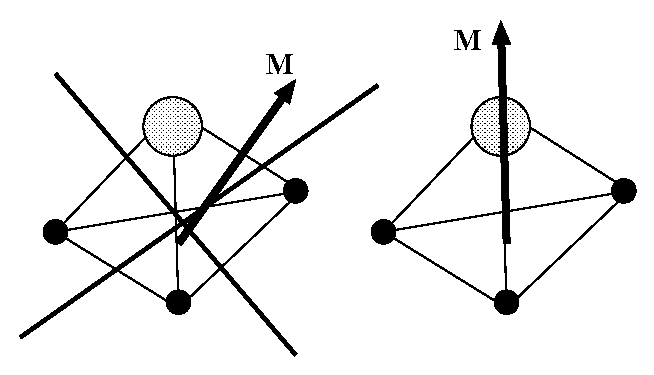
\includegraphics[scale=0.7]{pics/amonijak.eps}}

   \item tenzor vodljivosti ($j_i = \sigma_{ij}E_j$)
   \end{itemize}

\item ponekad je i pribliĹžna simetrija korisna
   
\end{enumerate}

\end{enumerate}

No, zašto je sustav simetričan? (Evolucioni razlozi? Biljke s pet latica
ne zaklanjaju tlo. Čovjek definiran gravitacijom i smjerom kretanja (ravnina),
a stablo samo gravitacijom (os). Zanimat će nas jednostavni sustavi.) 
$\Big\Downarrow$

\subsection*{2. Simetrije fizikalnih zakona}

\begin{enumerate}[-]

\item Newtonov zakon gravitacije
\[
      \vec{F}= G \frac{Mm}{r^3}\vec{r} \;,
\]
prividno nije simetričan na rotacije ($R:m\mapsto m$, ali $R:\vec{r}
\mapsto \vec{r}'\neq \vec{r}$), no on to zapravo jest jer se lijeva
i desna strana jednadĹžbe jednako transformiraju  --- nema preferiranog
usmjerenja u prostoru.

ZaĹĄto ne bi moglo biti:
\[
      F_x= G \frac{Mm}{r^2} \quad F_y = F_z =0 \;.
\]
To bi značilo da je $x$-smjer u prostoru drugačiji od ostala dva.
Sferna simetrija u običnom trodimenzionalnom prostoru se čini trivijalna,
ali na intuiciju i vizualizaciju se mnogo teže osloniti u slučaju 
simetrija kristala ili u slučaju sferne simetrije u
vektorskom prostoru kvantnomehaničkih stanja.

Rješenja sferno simetričnih Newtonovih jednadžbi gravitacije i mehanike
(npr. Sunčev sustav) nisu simetrična (zbog nesimetričnih početnih
uvjeta). Skup \emph{svih} rješenja je sferno simetričan.
(Zato je Newtonu bilo teĹĄko.)

\item znamo jedno rjeĹĄenje \Ra znamo i sva ona ostala koja iz 
 tog jednog dobijemo transformacijama simetrije

\item Ali, moĹžemo i bolje: sferna simetrija (centralna sila) \Ra
 $d\vec{L}/dt= d(\vec{r}\times\vec{p})/dt=0$ \Ra trajektorija je u ravnini;  
 \& Laplace-Runge-Lenzov vektor $d\vec{M}/dt=0$ \Ra  trajektorija
  je elipsa (bez rjeĹĄavanja diferencijalnih jednadĹžbi).

\item Slično za vodikov atom (ne moramo rješavati Schr\"{o}dingerovu
  jednadĹžbu) dobijemo
\[
     E_n =-\frac{R}{n^2}
\]
  (univerzalnost simetrijskih argumenata)

\end{enumerate}

Simetrija \Ra očuvani vektori $\Big\Downarrow$


\subsection*{3. Simetrije i zakoni očuvanja}

\begin{enumerate}[-]

\item $L$ ne ovisi o $q_i$ \Ra $L$ je simetričan
na transformacije koje mijenjaju $q_i$ 
\[
    \frac{\partial L}{\partial q_i}=\frac{d}{dt}\frac{\partial L}
{\partial \dot{q}_i}=0
\]
\Ra $p_i=\partial L/\partial\dot{q}_i$ je očuvan.(Noetherin teorem)

\item Očuvanje E, P, L, ... kao posljedica simetrije na translacije
 u vremenu, prostoru, rotacije, ... (prostorne simetrije)

\item Očuvanje naboja, barionskog broja, izospina, ... (interne simetrije)
\end{enumerate}

\subsection*{4. Principi simetrije koji određuju prirodne zakone}

Oblik Newtonovih zakona je samo djelomično određen zahtjevima
sferne simetrije. MoĹžemo li bolje?

\begin{enumerate}[-]

\item Specijalna teorija relativnosti: 
  (a) postulat relativnosti (b) svojstvo $c=const$ su iskazi
  određenih simetrija prostor-vremena. Iz njih je moguće izvesti
  čitavu teoriju.

\item simetrija na opće transformacije, princip ekvivalencije
  \Ra Einsteinova teorija gravitacije

\item Gell-Mannova interna simetrija i kvarkovi

\item Baždarna simetrija i teorije temeljnih međudjelovanja
\end{enumerate}
\end{document}
